\documentclass[oneside, noacknowlegments]{BYUPhys}
\usepackage{verbatim}
\usepackage{graphicx}
\usepackage{ragged2e}
\usepackage{amsmath}

% Your name
  \Author{Erik Swenson}

% Enter the date your thesis is approved
  \Year{2016}
  \Month{April}

% If you have a long title, split it between multiple lines using the \\ command
  \Title{Calcium and Hydrogen on Graphene as a Mechanism for 
  		 Hydrogen Storage}

% Your research advisor
\AdvisorTitle{Advisor}
  \Advisor{Bret Hess}

% For honors theses, enter the name of the honors Representative
  %\HonorsRepresentative{Kristine Hansen}

% The text of your abstract
  \Abstract{ Because of its status as an emerging energy carrier, methods of hydrogen storage are in high demand. Using computational methods, we explore a very large space of graphene structures with different adsorption configurations of hydrogen and calcium as mechanisms for hydrogen storage. We expand our search space further than the traditional search space by using cluster expansion to enumerate structures in a variety of computational cell shapes and sizes. This allows for periodicity not studied previously. We compare the results found using this type of enumeration with results obtained in other work and we present the most energetically favorable structures found in our search. }

 \Keywords{Hydrogen storage, cluster expansion, graphene}

% Acknowledge those who helped and supported you
  \Acknowledgments{
    [Acknowledgements should be simple, in good taste, and fit on one page]
  }

%% The members of your committee (masters only need A and B, PhD need all 4)
%  \MemberA{Committee Member A}
%  \MemberB{Committee Member B}
%  \MemberC{Committee Member C}
%  \MemberD{Committee Member D}
%

\begin{document}

 % Start page counting in roman numerals
 \frontmatter

 % This command makes the formal preliminary pages.
 % You can comment it out during the drafting process if you want to save paper.
\makepreliminarypages

% Make the table of contents.
\tableofcontents
 
% Create the list of figures.
\listoffigures

% Start regular page counting at page 1
\mainmatter

% OK. Everything is set up. Type your thesis here.

\chapter{Introduction}

\section{Motivation}
\label{sec:motivation}

In the search for a source of abundant, renewable, 
clean energy, molecular hydrogen as a fuel source has emerged as 
a promising alternative to hydrocarbons. Standard hydrocarbon fuel 
sources such as gasoline or propane give off $\mathrm{CO_2}$ as a 
byproduct. Both production and consumption of hydrocarbon fuels can 
pose a risk to the people or the environment in densely populated 
cities or highly industrialized areas where these activities are 
prominent. It is for this reason that hydrocarbon fuel is 
becoming less and less desirable in a world where the need for 
energy rapidly continues to grow.

We are not claiming that a molecular hydrogen fuel source will
completely solve this problem. After all, to \textit{produce} the
fuel, we somehow need to obtain and isolate the hydrogen molecules 
which requires some other energy source (\textit{e.g.} 
electricity). The \textit{consumption}, however, is much cleaner. 
When hydrocarbons are burned, $\mathrm{CO_{2}}$ is formed as the 
carbon bonds break and oxygenate. On the other hand, consumption of 
molecular hydrogen results in completely benign $\mathrm{H_{2}O}$ 
when the hydrogen bonds break and oxygenate, posing much less of a 
threat to the surrounding areas. The great advantage, then, of
hydrogen fuels comes when the production plants can be relocated
to remote areas outside the cities while only consumption occurs 
inside the cities. This somewhat isolates the inhabitants of the
cities from the harmful pollutants associated with fuel production.

Finding an efficient and practical way to store hydrogen in large
enough amounts for use as fuel now becomes the intriguing problem.
From a molecular perspective, we need a structure that is stable 
and binds molecular hydrogen, yet simple enough to manufacture 
in bulk amounts.

\section{Graphene and Hydrogen Storage}
\label{sec:graphene}

Graphene, an essentially two-dimensional hexagonal lattice of 
carbon atoms, was discovered in 2004 ~\cite{NovoselovGeim2004}. 
Graphene itself is incredibly strong, very thin, and an extremely 
good conductor of heat and electricty ~\cite{LeeWei2008}. The high 
density of potentially bond-forming atoms and the two-dimensional 
nature of the material make graphene a natural starting point for 
hydrogen storage applications ~\cite{Pumera2011}. In fact, 
graphene has already proven to bond with atomic hydrogen in the 
form of a derivative structure called \textit{graphane}
~\cite{SofoChaudhari2007, EliasNair2009}. This structure forms when 
a hydrogen atom bonds, or adsorbs, to each of the carbon atoms in 
the lattice. Throughout this paper, we will refer to any of these 
adsorption atoms bonded directly to the carbon monolayer as 
"adatoms".  In the graphane structure, the hydrogen atoms bond with 
both sides of the graphene sheet in an alternating top-bottom 
fashion (see Figure \ref{fig:GraphaneDiagram}). A slight "buckling" 
is introduced to the lattice as a result of this bonding.

\begin{figure}
	\centering
	\begin{minipage}[Test 1]{0.475\textwidth}
		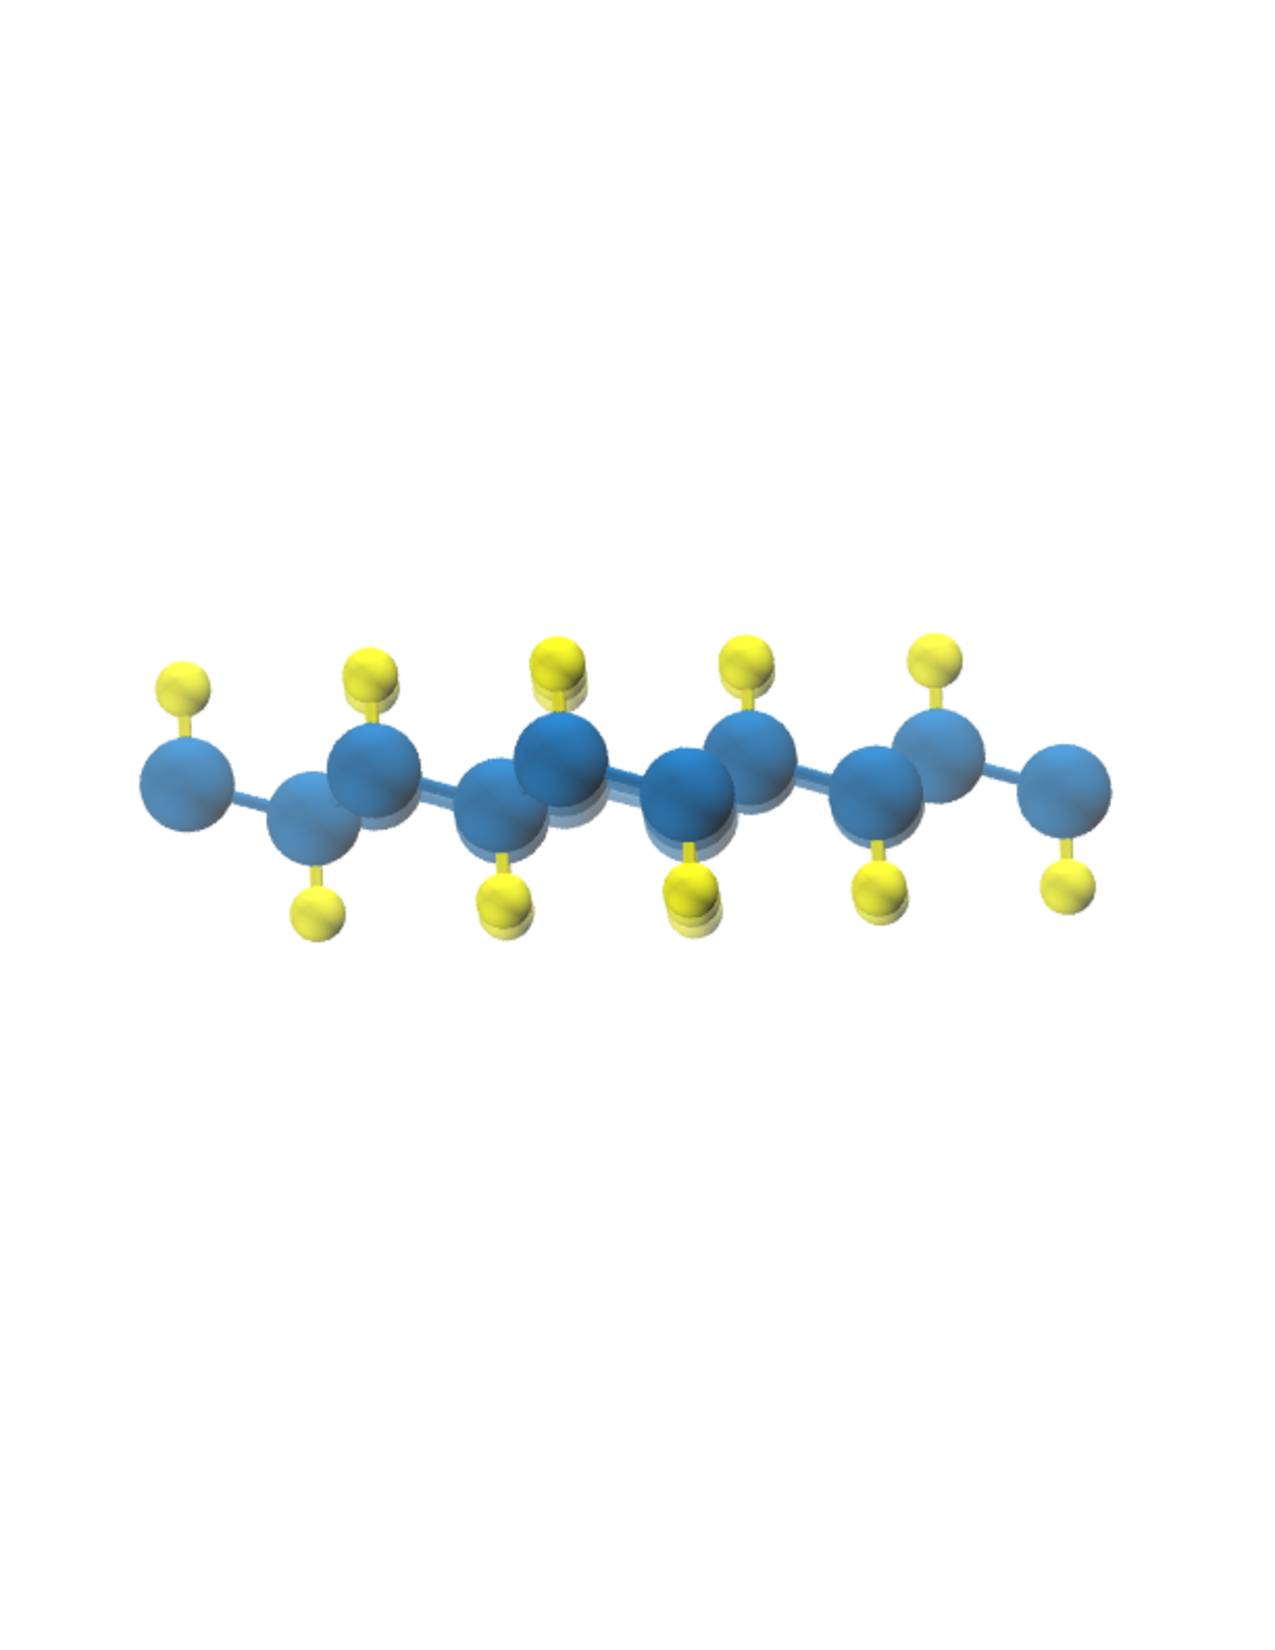
\includegraphics[width=\textwidth]
			{graphane_diagram_cropped}
		\centering \textit{(a)} Side View
	\end{minipage}
	\hfill
	\begin{minipage}[Test 2]{0.475\textwidth}
		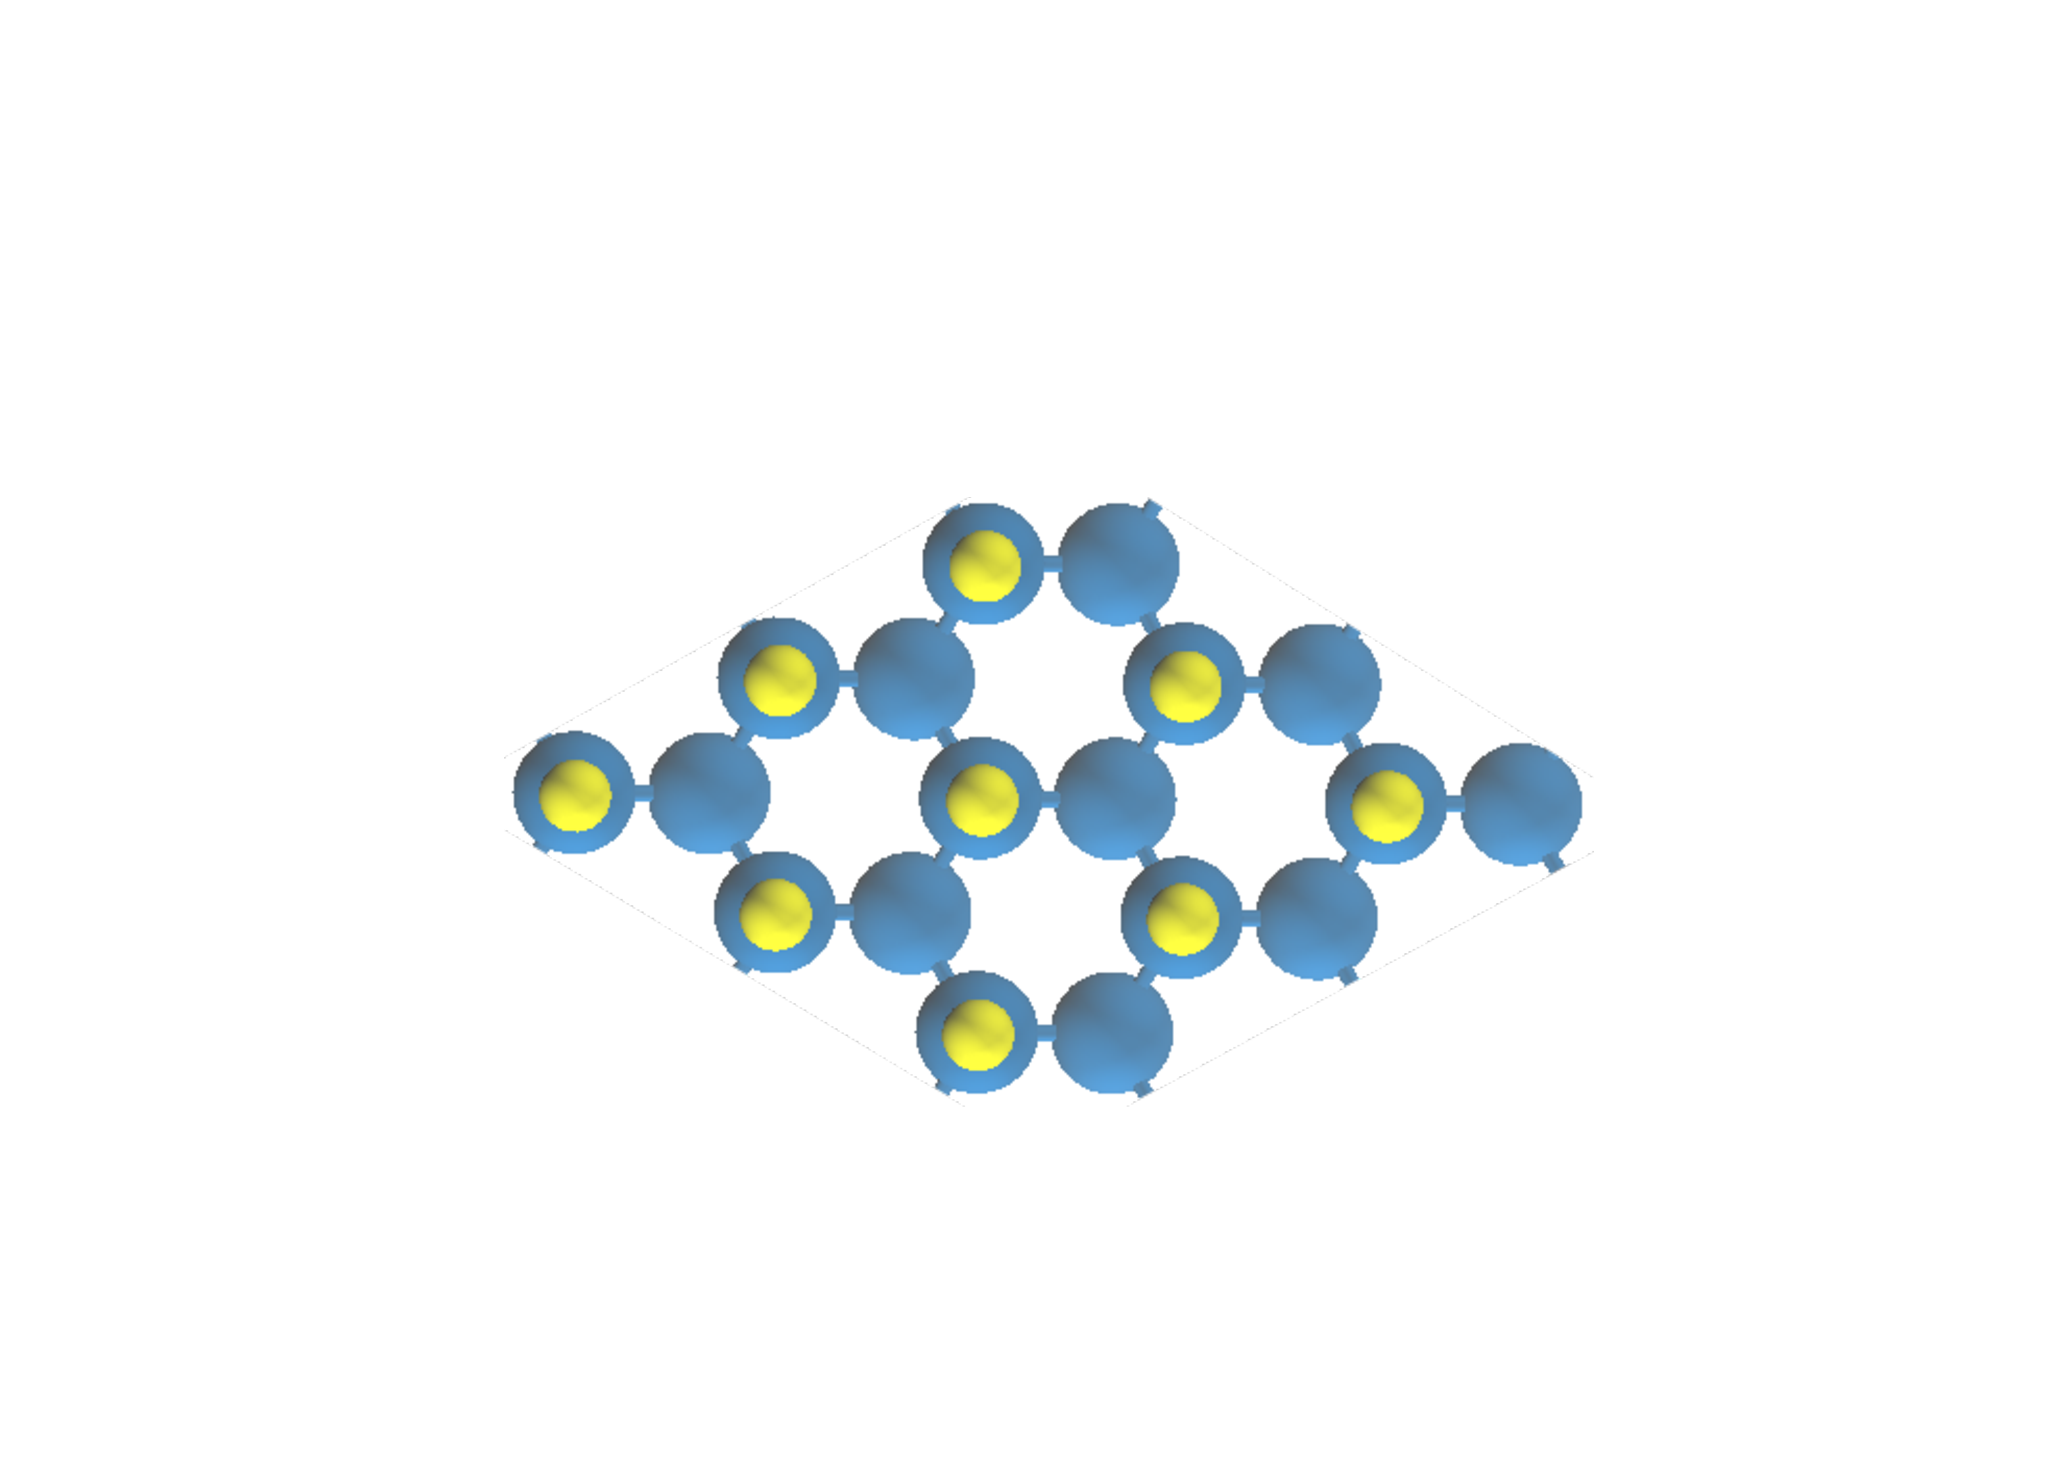
\includegraphics[width=\textwidth]{graphane_diagram_top}	\\
		\centering \textit{(b)} Top View
	\end{minipage}
	\raggedright
	\caption{Diagram of Graphane Structure}
	{\label{fig:GraphaneDiagram}	A visual depiction of the graphane 
	 structure. Note the alternating above-below scheme and lattice 
	 buckling apparent in \textit{(a)}.}
\end{figure}

However, graphane by itself is not very useful for hydrogen storage 
even though it provides a hydrogen atom for every carbon atom in 
the lattice. Graphane is a very stable structure which makes 
extracting the hydrogen atoms an energy consuming task. To break 
the strong, covalent bonds ($\sim$6.56 eV / atom 
~\cite{SofoChaudhari2007}) that have formed between the carbon and 
hydrogen atoms, we would have to heat the structure---again drawing 
from another energy source---to the point that the energy lost 
balances the energy gained.  Even if there was some way to easily 
extract the hydrogen atoms, they would tend to form bonds with each 
other as soon as they were far enough away from the carbon 
monolayer, releasing the energy we want to harvest during the 
formation of the $\mathrm{H_{2}}$ bond.  All that aside, atomic 
hydrogen (H) is much less useful as a fuel source than molecular 
hydrogen ($\mathrm{H_{2}}$).  We need a structure that binds pre-
formed hydrogen molecules and, because of its stability, graphane 
does not.

We can remedy this problem by making a small modification to the 
graphane structure. If we replace some of the hydrogen adatoms with 
metal atoms, we can create a structure that might bind a reasonable 
amount of molecular hydrogen. 

Computational work has already performed examining calcium and 
lithium as the adatoms with promising results. Hussain \textit{et 
al.} have explored both of these metals and report a hydrogen 
storage capacity of 6 wt. \% for calcium~\cite{HussainPathak2012} 
and 12 wt. \% for lithium~\cite{HussainDeSarkar2012, 
HussainMaark2012, HussainDeSarkar2014, HussainPathak2011}, both 
with reasonable adsorption energies.

\section{Our Project}
\label{sec:our_project}

In this paper, we also explore computationally the possibility of 
using a graphene monolayer doped with calcium and hydrogen as a 
practical solution to the hydrogen storage problem. However, our 
work goes beyond the work that has previously been carried out in 
two ways. 

Firstly, we allow for "vacancies"---carbon sites with no 
corresponding atom in the adsorbant monolayer.  With vacancies in 
the structure, the adatoms may have the ability to interact with 
more of the carbon atoms, producing higher binding energies between 
the carbon layer and the adatom layer.  More space between the 
adatoms might also reduce the tendency to cluster, a persistent 
plague in the hydrogen storage field.

Secondly, we examine structures from a multitude of computational 
(unit) cell sizes and shapes. This adds a significant degree of 
complexity to structure enumeration, but other members of our group 
have developed methods to speed up the computation. Traditionally, 
only one diamond-shaped unit cell has been studied which greatly 
limits the possible atomic configurations that can be acheived.  We 
use the UNiversal CLuster Expansion (UNCLE)~\cite{LerchUNCLE} code 
to enumerate many different cell shapes that contain the same 
number of atoms as the traditional unit cell (see Figure 
\ref{fig:unit_cells}).  By using this type of structure 
enumeration, we hope to discover new structures with promising 
energetics.

\begin{figure}
	\centering
	\begin{minipage}{0.475\textwidth}
		\centering \textit{(a)} Volume 4 ($2\times2$)
		\includegraphics[width=\textwidth]
			{unit_cell_plots/77}
	\end{minipage}
	\hfill
	\begin{minipage}{0.475\textwidth}
		\centering \textit{(b)} Volume 5 ($1\times5$)
		\includegraphics[width=\textwidth]{unit_cell_plots/96}
	\end{minipage}
	\\ \bigskip
	\begin{minipage}{0.475\textwidth}
		\centering \textit{(c)} Volume 7 ($1\times7$)
		\includegraphics[width=\textwidth]
			{unit_cell_plots/849}
	\end{minipage}
	\hfill
	\begin{minipage}{0.475\textwidth}
		\centering \textit{(d)} Volume 9 ($3\times3$)
		\includegraphics[width=\textwidth]{unit_cell_plots/11130}	\\
	\end{minipage}
	\raggedright
	\caption{Examples of the different computational unit cells 
		used in structure enumeration. The cells are defined by 
		the periodic black lines in the drawings. The blue circles 
		represent carbon atoms in the graphene lattice. Yellow and 
		red circles represent hydrogen and calcium adatoms 
		respectively. A thick border around an adatom signifies 
		that the atom is below the plane. Note that the structure 
		in \textit{(d)} is a two-dimensional representation of the 
		same structure pictured in Figure 
		\ref{fig:GraphaneDiagram}.}
	\label{fig:unit_cells}
\end{figure}

We begin by briefly summarizing some key concepts and providing 
definitions for important terms. We will outline the computational 
algorithms used for structure enumeration, selection, and 
prioritization. We conclude with a presentation of the results we
obtained. We compare structures with no vacancies against 
structures with vacancies and analyze what we find by searching a 
variety of cell shapes and sizes. We also make mention of several 
directions for future work in the field, many of which are 
currently being explored by our group. 

\chapter{Methods}

\section{Methods Common to Other Groups}
\label{sec:common_methods}

\subsection{Density Functional Theory}

We ran simulations using the Vienna Ab-Initio Simulations Package 
(VASP)~\cite{KresseMDLiqMetals, KresseMDGermanium, 
KresseEfficiencyPWBasis, KresseIterativeSchemes} code which peforms 
calculations based on Density Functional Theory (DFT). DFT, as the 
name suggests, uses functionals of electron density to model atoms 
and their interactions (citation). In the simplest of terms, a
\textit{functional} is a function of another function. In other 
words, it is a function that takes in a vector and maps it to a 
scalar. In the case of modeling molecular structure energetics, the 
energy functional is of greatest interest. It takes in the electron 
density function at a given point and returns a scalar energy 
value. To find energetically favorable structures, then, the goal 
is to minimize the energy functional for each 
structure. 

A drawback to DFT is that it is somewhat inaccurate in the 
calculation of weak van Der Waals forces which play a large role in 
the carbon-hydrogen-metal systems being studied (citation). At the 
heart of this problem is the fact that VASP makes use of two 
notable approximations to increase computational speed. In the 
Local Density Approximation (LDA), the energy functional only 
depends on the density at the point where the functional is being 
evaluated. A slightly modified approach called the Generalized 
Gradient Approximation (GGA) is similar except that it also takes 
into account the gradient of the density at the point being 
evaluated. Both of these approximations have been shown to 
inaccurately represent the van Der Waals interactions, with LDA 
overestimating and GGA underestimating.~\cite{HussainPathak2012} 
That being said, for simulations with more than just a few atoms, 
these methods are industry standards and the best that we can do.

\subsection{Cluster Expansion}

Cluster Expansion (CE) provides a mathematical model from which we 
can predict the energies of a comprehensive space of structures 
based on the calculated energies of a few structures. CE gets its 
name from the "clusters", or combinations of occupied sites, that 
are summed together to represent a structure. Each cluster has an 
associated weight term which represents energy in this case. 
Clusters and their weights model the interaction between the atoms 
that make up the cluster. Clusters can be defined by a single 
atom (a 1-body cluster) or include any number of atoms in the 
lattice (an \textit{n}-body cluster). As we include more clusters, 
the accuracy of the model increases until, in the limit of 
including all possible structures, it approaches the actual energy 
of the structure. However, we can obtain excellent results even 
with a significant truncation. UNCLE truncates the expansion after 
6-body clusters.

\begin{comment}
Include some sort of explanation of the difference between the 
lattice and the sites where the atoms are located.  Symmetry is 
really what defines the lattice.  For our case, we deal with a 
hexagonal lattice because we only have to rotate the lattice 60 
degrees to obtain an identical lattice.
\end{comment} 

The cluster expansion model is defined by the following equation:		
	\begin{equation} \label{ce_summation}
		E_{\sigma}=\sum_{c}{\Pi_{\sigma c}J_{c}} 
	\end{equation}
where $\sigma$ represents a particular structure and $c$ represents 
a particular cluster. The $E_{\sigma}$ term represents the known 
(calculated) energy of the structure $\sigma$. The $\Pi$ matrix is 
a matrix of correlation values between structures and clusters. The 
rows in the matrix represent structures and the columns represent 
clusters. Finally, the $J_c$ term is an energy "weight" for a given 
cluster. For visualization's sake, it may be easier to understand 
in matrix form.
	\begin{equation} \label{ce_matrix}
		\begin{bmatrix}
			E_1 \\
			E_2 \\
			\vdots \\
			E_n
		\end{bmatrix}
		=
		\begin{bmatrix}
			\Pi_{11} & \Pi_{12} & \cdots & \Pi_{1m} \\
			\Pi_{21} & \Pi_{22} & \cdots & \Pi_{2m} \\
			\vdots   & \vdots   & \ddots & \vdots \\
			\Pi_{n1} & \Pi_{n2} & \cdots & \Pi_{nm}
		\end{bmatrix}
		\begin{bmatrix}
			J_1 \\
			J_2 \\
			\vdots \\
			J_m
		\end{bmatrix}
	\end{equation}
In other words, the energy of a given structure is simply the sum 
of the properly weighted terms in the row of the $\Pi$ matrix that 
represents the structure. If the $\Pi$ matrix were square, we could 
simply invert the matrix and multiply to find the weights. However, 
the number of clusters and the number of structures do not have to 
be (and rarely are) equivalent. This generally results in a an 
underdetermined system for our purposes and more complex linear 
algebra techniques are required to solve it. Fortunately, Nelson 
\textit{et al.} have developed Bayesian Compressed Sensing methods 
to solve this system efficiently.~\cite{NelsonCE}

Once the weights are found, the multiplication on the right side of 
Eq. \ref{ce_summation} predicts the energy for any structure in the 
space.

\section{Enumeration of Structures}

We use the UNCLE code to perform enumeration of all possible 
symmetrically inequivalent structures in a given space. UNCLE 
performs a solely mathematical enumeration based on the shape of 
the lattice and the adatom options at each lattice site. This type 
of enumeration will inevitably produce structures that could not 
possibly exist in nature due to the size of the adatoms. For 
example, because the atomic radius of a calcium atom is large ($
\sim$1.74 \AA) and carbon-carbon bond lengths in the graphene 
lattice are not ($\sim$1.42 \AA), we cannot place two calcium atoms 
adjacent to one another. Pairs of atoms that cannot be placed next 
to each other are termed \textit{forbidden pairs}. We do not want 
to waste time in the search running "forbidden" structures through 
VASP calculations so, to this end, other members of our group have 
added functionality to exclude them from the enumeration (reference 
Joseph's paper). 

Our enumeration, however, is left somewhat incomplete. From sets of 
structures that are rotationally or translationally equivalent 
(like 10 and 01) we only keep one. We then use \textit{tiles} of 
the remaining symmetrically inequivalent structures to build up our 
computational unit cells. Because we form the tiles after 
elimination by symmetry, some tiles are not available for use and, 
thus, some structures are left out of the enumeration. This does 
have a positive consequence, though, in that we can perform higher 
volume enumerations and explore higher volume structures in our 
search than we could otherwise.

\section{Search for Favorable Structures}

The main portion of my work in the group dealt with creating, 
coding, and automating the iterative process of searching the space 
of possible structures. The basic algorithm can be seen in Figure 
\ref{fig:ProcessDiagram}. It starts by selecting a set of what are 
called independently and identically distributed (IID) structures 
to use as initial input to the iteration loop. IID means that the 
initial set will include structures that are as different as 
possible from one another.

\begin{figure}
    \centerline{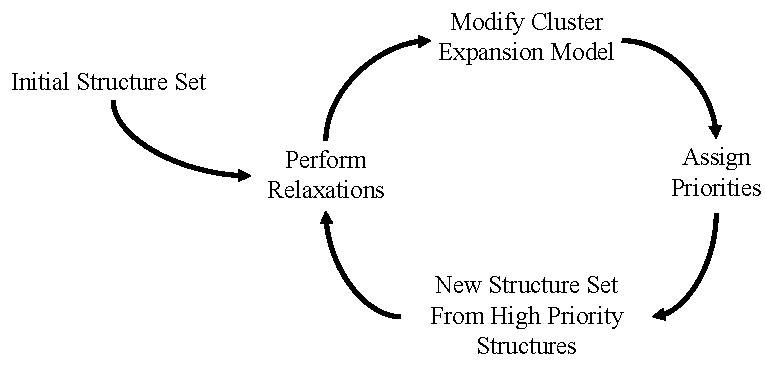
\includegraphics{Erik_Swenson_Schematic}}
    \caption{A high level map of the iteration process. We start 
    		with a randomly selected set of structures. We run the 
    		structures through atomic and electronic relaxation 
    		routines and use that data to create a predictive model for 
    		all possible structures. We then assign each structure a 
    		priority and choose a set of highest priority to run back 
    		through the loop.}
	\label{fig:ProcessDiagram}
\end{figure}

Our new code takes the IID structure set and extracts the important 
information into a format that VASP can work with. VASP iteratively 
makes slight adjustments to the positions of the ions and the 
electrons in order to minimize the energy of the structure in a 
process called \textit{relaxation}. 

Once VASP has found the energy-minimized configuration for each 
structure, we create a CE model based on the results from this 
initial structure set. The model predicts the energy of all the 
structures in the space. (Initially, this model is not very 
accurate, but as we add more structures to the model each 
iteration, the accuracy increases substantially.) We prioritize the 
structures according to a decaying exponential scale. Energetically 
favorable (low energy) structures are given high priority while 
high energy structures are given a much lower priority.

We then select a new set of the highest priority structures from 
the pool of structures that have not been run through VASP 
calculations and the loop begins again. It should be noted that, 
because we choose new structures at the end of each iteration based 
on their priority, the energy-predictive model we refine may not be 
very accurate for higher energy structures. This is not an issue 
since high energy structures are of no practical interest to us 
anyway. 

\chapter{Results}

\section{Energy Metrics}

When analyzing the results of our energy calculations, the most 
intuitive metric we use to summarize a structure's energy is what 
we have termed formation energy. Formation energy (FE) is defined 
as the average energy per atom required to pull an adatom out of a 
reference structure containing only that particular atom and bind 
it to the graphene layer. For hydrogen, we use a hydrogen molecule 
($\mathrm{H_{2}}$) as the reference structure and for calcium, the 
reference structure is a hexagonal monolayer of Ca atoms bound 
together. Mathematically,
	\begin{equation} \label{form_E}
		FE_{struct} = E_{struct} - \left(E_{graphene} + \sum_{i}
		{N_{i}E_{i}^{ref}}\right)
	\end{equation}
where $E_{struct}$ is the energy value of that structure directly 
from the calculations, $E_{graphene}$ is the calculated reference 
energy of the graphene, and the summation term gives the number of 
each type of adatom multiplied by its corresponding reference 
energy.

Another important metric used in our analysis is planar binding 
energy (PBE) which, in the most simple terms, tells us how much 
energy is required to separate the adatom layer from the carbon 
monolayer far enough that the interaction between the two layers is 
negligible. Structures with positive or weakly negative PBE are 
essentially already separated into layers. Mathematically,
	\begin{equation} \label{pbE}
		PBE_{struct} = E_{struct} - \left(E_{graphene} + 
		E_{adatoms}\right) 
	\end{equation}
where $E_{struct}$ and $E_{graphene}$ carry the same meaning as in 
FE and $E_{adatoms}$ represents the total energy of the isolated 
adatom layer.

Our goal is to find structures that exhibit a strong FE as well as 
a strong PBE. To this end, we have defined a third, non-physical 
quantity called sorting energy (SE) which is defined as 
	\begin{equation} \label{inter_E}
		SE_{struct} = max\left(FE_{struct}, PBE_{struct}\right)
		\quad.
	\end{equation}
When we sort the structures according to their SE, we can easily 
find those that have strong FE as well as PBE.

Figure \ref{fig:FEvsPBE} shows a plot of PBE vs. FE for volume nine 
structures where vacancies are allowed. We can see that the region 
of interest representing structures that simultaneously boast low 
FE and PBE is very sparsely populated. In fact, the small trail of 
structures on the far left hand side that dip down into this region 
are all "graphane-like" in that they only contain hydrogen atoms 
bonded to the carbon monolayer. Since these structures have no 
calcium content and, hence, no way to bind hydrogen molecules, they 
are of no practical interest to us for hydrogen storage 
applications. Our focus will be on the other structures that border 
this empty region even though their overall energetics may be 
higher than we had hoped for.

\begin{figure}
	\centering
	\begin{minipage}{0.65\textwidth}
		\centering
		\includegraphics[width=\textwidth]{FEvsPBE_2}
	\end{minipage}
	\caption{A plot of formation energy vs. planar binding energy 
		for volume 9 double-sided structures. Each blue dot 
		represents a particular structure. Ignoring the tail of 
		"graphane-like" structures at the far left side of the 
		plot, note the large gap in the region of strong FE and PBE 
		where very desirable structures would appear.}
	\label{fig:FEvsPBE}
\end{figure}

\section{Single-Sided Bonding}

In the single-sided case, we find many structures with strong FE as well as PBE.  The structures with the lowest SE, however, contain high calcium concentrations and show signs of clustering perpendicular to the carbon monolayer rather than binding directly to the monolayer. This is not too surprising for single-sided bonding since we would expect calcium atoms that are in close proximity to each other to form bonds of their own rather than with the carbon atoms. 

Calcium clustering causes two main problems. Firstly, the clustered calcium atoms create strong bonds with each other, reducing the ability to bind $\mathrm{H_{2}}$ to the structure. Secondly, even if the calcium clusters could still bind $\mathrm{H_{2}}$, the cluster takes up more space, resulting in a much less space-efficient structure for hydrogen storage.

The lowest energy single-sided structure found in our search that did not suffer from calcium clustering is shown in Figure \ref{fig:SLowest}. We will call this structure S1. The calcium atoms in S1 are spaced far enough apart so as to avoid interacting too strongly with each other. Table \ref{form_energy_tab} shows the four lowest energy structures in the single-sided search excluding graphane-like structures and structures that suffer from calcium clustering. Notice that these structures all have FE in the range of $\sim -0.8$ eV and PBE in the range of $\sim -2.3$ eV with the exception of structure S4 having $\mathrm{PBE} = -2.899$ eV.

\begin{figure}
	\centering
	\begin{minipage}{0.5\textwidth}
		\centering
		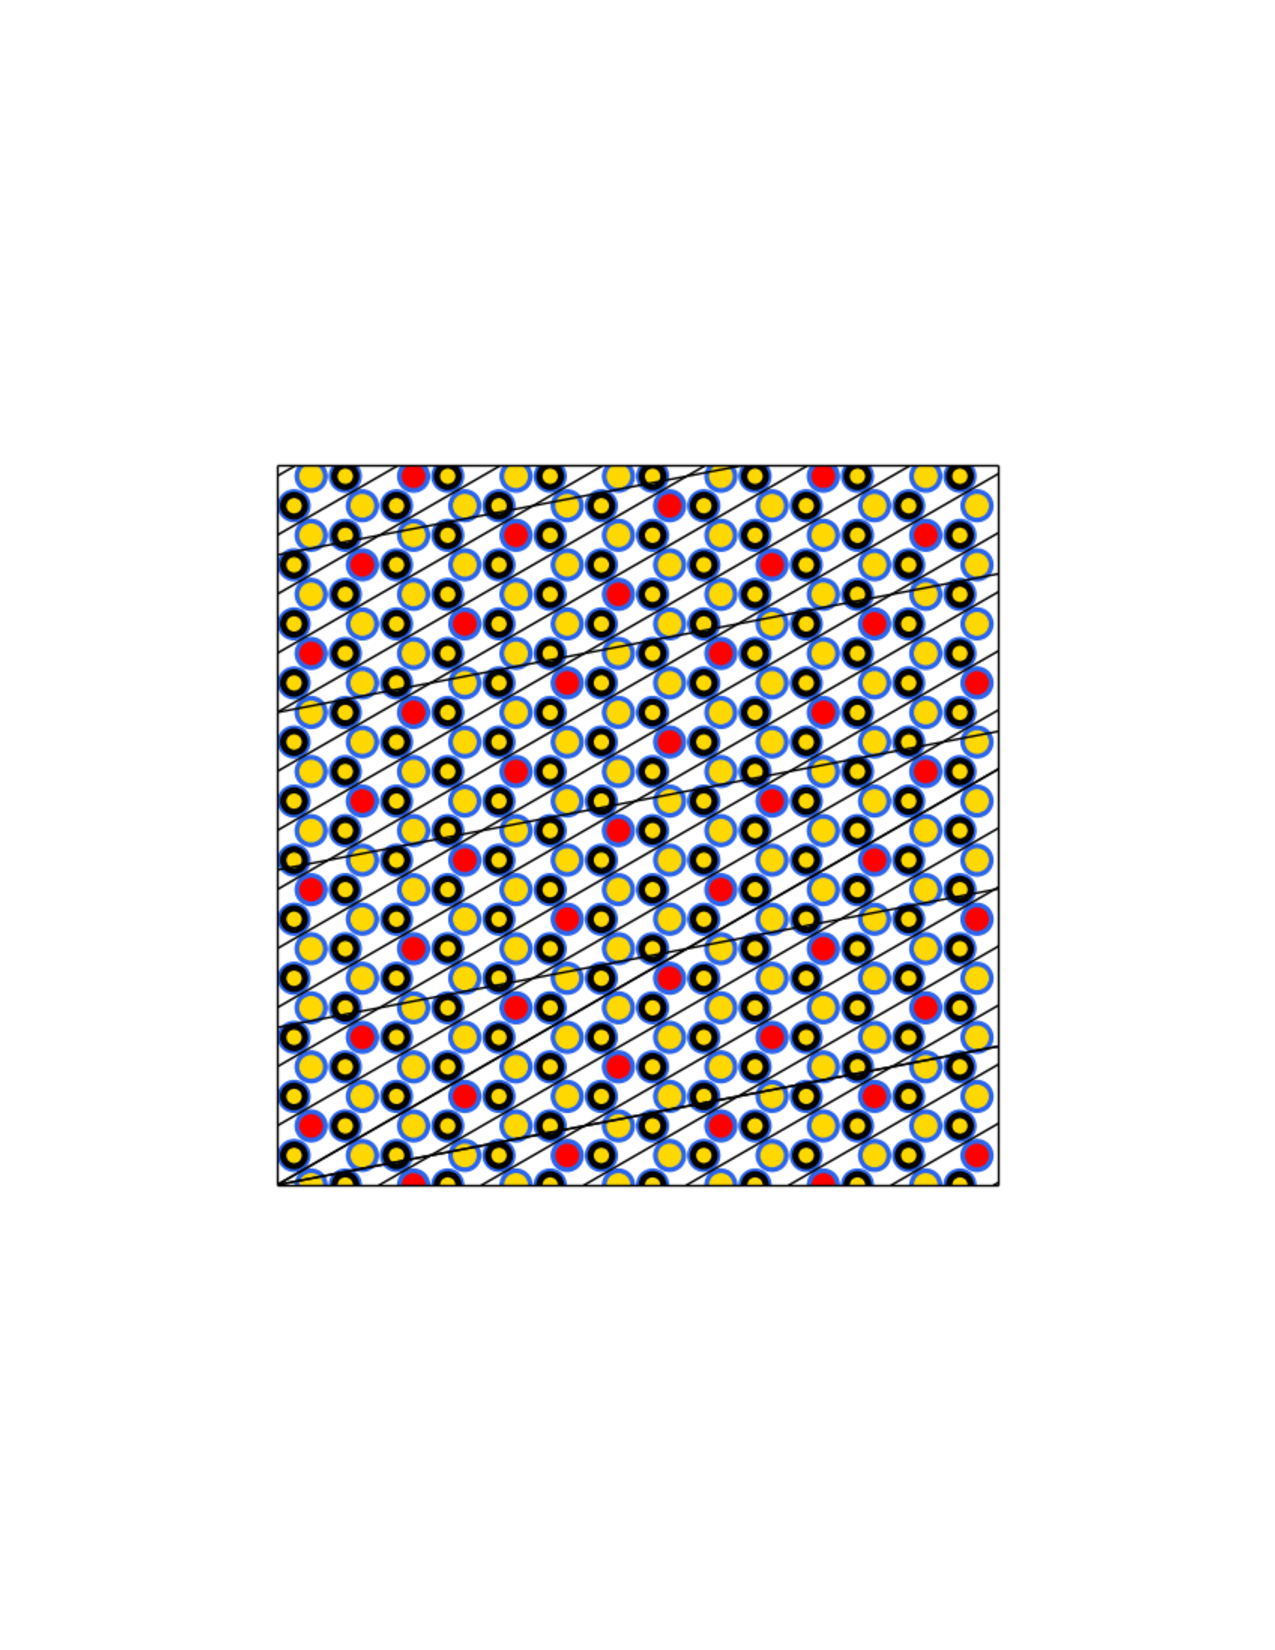
\includegraphics[width=\textwidth]{212}
	\end{minipage}
	\caption{Structure S1, the lowest energy structure in the 
		single-sided search that contains calcium atoms and does 
		not suffer from calcium clustering.}
	\label{fig:SLowest}
\end{figure}

\begin{table}
	\footnotesize
	\centering
	\begin{tabular}{lcccc}
	\hline
	\hline
	Structure & Volume & SE & FE & PBE \\
	& & (eV / atom) & (eV / atom) & (eV / atom) \\
	\hline
	S1 & 8 & -0.815 & -0.815 & -2.271 \\
	S2 & 8 & -0.806 & -0.806 & -2.322 \\
	S3 & 8 & -0.804 & -0.804 & -2.316 \\
	S4 & 8 & -0.804 & -0.804 & -2.899 \\
	\hline
	\hline
	\end{tabular}
	\caption{The four structures with the lowest sorting energy for 
		a single-sided H-Ca system.}
	\label{form_energy_tab}
\end{table}

\section{Double-Sided Bonding}

[\textit{Insert results from binary double-sided bonding and compare with the structure from the paper.}]

\section{Effect of Vacancies}

[\textit{Insert results from ternary single-sided and compare with binary single-sided.}]

[\textit{Insert results from ternary double-sided and compare with binary double-sided.}]

[\textit{This is made up, but it would be really cool.}] The comparisons made above, show that vacancies play an important role in the formation of structures for hydrogen storage. We have shown that vacancies allow for higher concentrations of calcium atoms without giving way to clustering. This is a desirable characteristic because, theoretically, structures with a higher concentration of calcium should be able to bind more hydrogen and, therefore, be better suited to hydrogen storage applications.

\section{Variation of Unit Cells}

It is clear that the size and shape of the computational unit cell used is an important parameter in the search for low energy structures. In the single-sided search not allowing vacancies---the search where having a large cell size should matter the most---the highest ranking of any structure of the $3 \times 3$ unit cell type pictured in Figure \ref{fig:unit_cells} \textit{(d)} was $\mathrm{29}^{th}$. Out of the 100 lowest energy structures in the search, only \textit{30} were volume nine structures and, of those thirty, only \textit{eight} had $3 \times 3$ unit cells. Interestingly enough, 49 of the lowest 100 came from volume eight unit cells. Most of the low energy structures had a longer, stretched unit cell like the one pictured in Figure \ref{fig:unit_cells} \textit{(c)}. This is probably because spreading the calcium atoms out farther from each other decreases their interaction with each other and increases their interaction with the graphene monolayer. 

This result strongly suggests that the periodicities encompassed by the volume nine, $3 \times 3$ unit cell are not ideal periodicities for a H-Ca system. In any case, it is an important illustration of the fact that, in order to perform a complete search of the space, the size and shape of the unit cell must be a parameter in the search.

% Start labeling chapters with letters and calling them appendices
\begin{appendices}

\chapter{Appendix Title}
\label{sec:appendixname}

You can put supplimentary content in an appendix.

\end{appendices}

% Make the bibliography.
% Enter your references in the BibTex file "references.bib"
\bibliography{references}

% Make the index
 \printindex

\end{document}
